\subsection{Abscis van een punt op een geijkte rechte}

De verzameling $\mathbb{R}$ van de re\"ele getallen kun je voorstellen als de verzameling van de punten op een geijkte rechte.
Een geijkte rechte is een rechte $l$ waarop een paar van 2 verschillende punten $(A;B)$ gekozen is.
De volgorde van zulke punten heeft belang.
Het eerste punt $A$ heet de oorsprong van de ijk.
Deze oorsprong komt overeen met het getal 0.
Het tweede punt $B$ komt overeen met het getal 1.

\begin{figure}[h]
\begin{center}
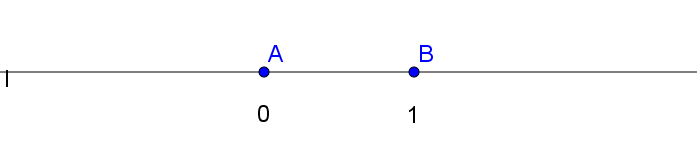
\includegraphics[height=2 cm]{4_opp_inhoud_an_meetk/inputs/AMTekst1Fig1}
\end{center}
\end{figure}

De richting van $A$ naar $B$ noem je de positieve richting van de geijkte rechte.
Omdat op $l$ door de ijk een positieve richting gedefinieerd is noem je $l$ ook een geori\"enteerde rechte.
Die ori\"entatie duidt je vaak aan met een pijl.
Je stelt een geori\"enteerde rechte ook voor zoals op volgende tekening.

\begin{figure}[h]
\begin{center}
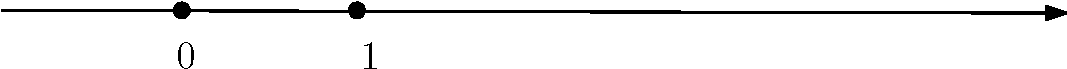
\includegraphics[height=7 mm]{4_opp_inhoud_an_meetk/inputs/AMTekst1Fig2}
\end{center}
\end{figure}

Een natuurlijk getal $n$ (bijvoorbeeld 3) komt overeen met het punt $C$ op $l$ langs dezelfde kant van $A$ als het punt $B$ door $n$ keer vanuit $A$ de afstand van $A$ naar $B$ af te passen.
Je ziet dit ge\"illustreert voor $n=3$.

\begin{figure}[h]
\begin{center}
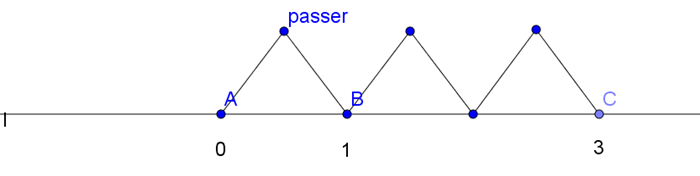
\includegraphics[height=2 cm]{4_opp_inhoud_an_meetk/inputs/AMTekst1Fig3}
\end{center}
\end{figure}

%Voor de makers: mijn voorstel is dit uit voor te doen met passer gefilmd door een topcamera.
%Met passer van $A$ naar $B$ afpassen.
%Dit daarna vanuit B naar rechts afpassen (dat geeft op de rechte het niet benoemde punt).
%En van daaruit nog eens naar rechts afpassen (dat geeft dan het punt C). \vspace{5mm}

\subsubsection{Rationaal getal}

Een rationaal getal gegeven door een positieve breuk $\frac{n}{m}$ stel je als volgt voor door een punt $C$ op $l$.
Je verdeelt het lijnstuk van $A$ naar $B$ in $m$ gelijke delen (je ziet straks hoe je dat kunt construeren).
Noem $B'$ het eerste deelpunt na $A$.
Als $n=a+\frac{n'}{m}$ met $0<n'<m$ en $a$ een natuurlijk getal, dan duidt je eerst het punt $C'$ aan op $l$ dat overeenkomt met het natuurlijke getal $a$.
Vervolgens pas je vanuit $C'$ in de positieve richting $n'$ keer de afstand van $A$ naar $B'$ af.
Dit is het punt $C$.

Je ziet dit ge\"illustreerd voor $\frac{n}{m}=\frac{11}{4}=2+\frac{3}{4}$ (dus $a=2$ en $n'=3$).\vspace{5mm}

%Voor de makers: mijn voorstel is ook dit voor te doen met passer en lineaal door een topcamera.
%Je start met de geijkte rechte waar $A$ en $B$ op liggen.
%Je tekent door $A$ de tweede snijdende rechte en kiest daarop een ijk $(A;B_0)$.
%Met de passer pas je op de rechte het punt $Q_0$ af dat met 4 overeen komt. Dat geeft als resultaat de eerste figuur.

%Vervolgens wordt het lijnstuk $Q_0B$ getekend en door met evenwijdig lijnstukken daaraan te werken bekomt men de verdeling van $A$ naar $B$ in 4 gelijke delen.
%(Evenwijdige rechten kun je tekenen door een lineaal en een winkelhaak (rechthoekige driehoek) die je over dat lineaal verschuift)
%Dit geeft dan het punt $B'$ en het resultaat is de tweede figuur.
%
%Tenslotte wordt door het afpassen met de passer (index 1) eerst het punt $C'$ gevonden en daarna door afpassen met de passer (index 2) het punt $C$.

\subsubsection{Negatief getal}

%\begin{figure}[h]
%	\begin{center}
%		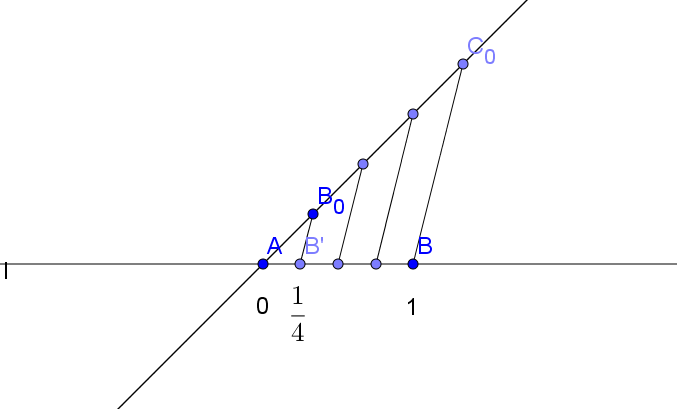
\includegraphics[height=2 cm]{4_opp_inhoud_an_meetk/inputs/AMTekst1Fig5}
%	\end{center}
%\end{figure}
%
%\begin{figure}[h]
%	\begin{center}
%		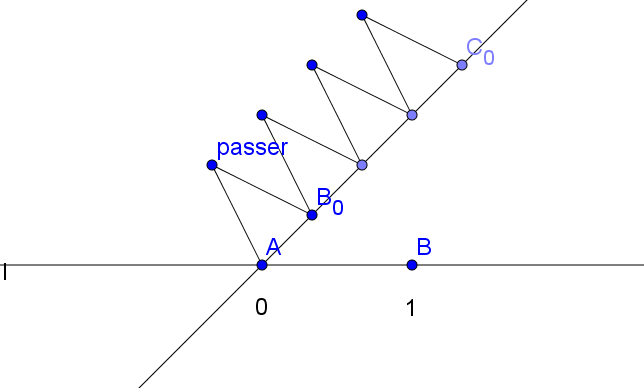
\includegraphics[height=2 cm]{4_opp_inhoud_an_meetk/inputs/AMTekst1Fig4}
%	\end{center}
%\end{figure}

%\begin{figure}[h]
%\begin{center}
%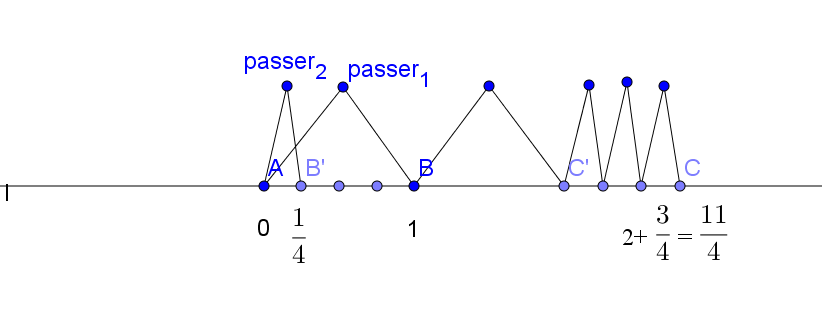
\includegraphics[height=2 cm]{4_opp_inhoud_an_meetk/inputs/AMTekst1Fig6}
%\end{center}
%\end{figure}

Een negatief geheel getal of een negatief rationaal getal construeer je door afstanden af te passen naar de negatieve richting van de geijkte rechte $l$.

\subsubsection{Re\"eel getal}

Met veel meer geavanceerde wiskunde kan aangetoond worden dat ieder re\"eel getal (kommagetal) overeenkomt met een punt van $l$ en dat ieder punt van $l$ ook overeenkomt met een re\"eel getal. Een geijkte rechte is daardoor een meetkundige voorstelling van de verzameling $\mathbb{R}$ van de re\"ele getallen.\vspace{2mm}

Door gebruik te maken van de Stelling van Pythagoras kun je bijvoorbeeld ook het punt van $l$ dat overeenkomt met een vierkantswortels uit een natuurlijk getal construeren.
Je ziet dit ge\"illustreerd voor $\sqrt{5}$.
Je gebruikt daarbij dan $\sqrt{5}$ de schuine zijde is van een rechthoekige driehoek met rechthoekszijden 1 en 2.\vspace{5mm}

%Voorde makers: mijn voorstel is ook dit te voor te doen met passer en lineaal door een topcamera.
Je start met de geijkte rechte waar $A$ en $B$ op liggen.
Loodrecht (winkelhaak) op $l$ door $B$ trek je een rechte en daarop pas je met passer tweemaal vanuit $B$ de afstand van $A$ tot $B$ af.
Dit geeft het punt $B'$ en het resultaat is te zien in Figuur \ref{4.2.1_fig_reeel_fig1}.

Met de passer met middelpunt $A$ en straal de afstand van $A$ tot $B'$ maak je een cirkelboog die op $l$ het punt $C$ geeft.
Het resultaat is te zien in Figuur \ref{4.2.1_fig_reeel_fig2}.

\begin{figure}[h]
\begin{center}
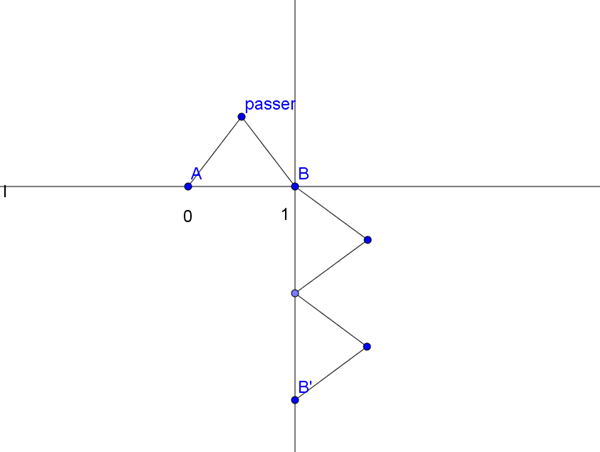
\includegraphics[width=.5\linewidth]{4_opp_inhoud_an_meetk/inputs/AMTekst1Fig7}
\caption{Constructie vierkantswortel van een natuurlijk getal (1).}
\label{4.2.1_fig_reeel_fig1}
\end{center}
\end{figure}

\begin{figure}[h]
\begin{center}
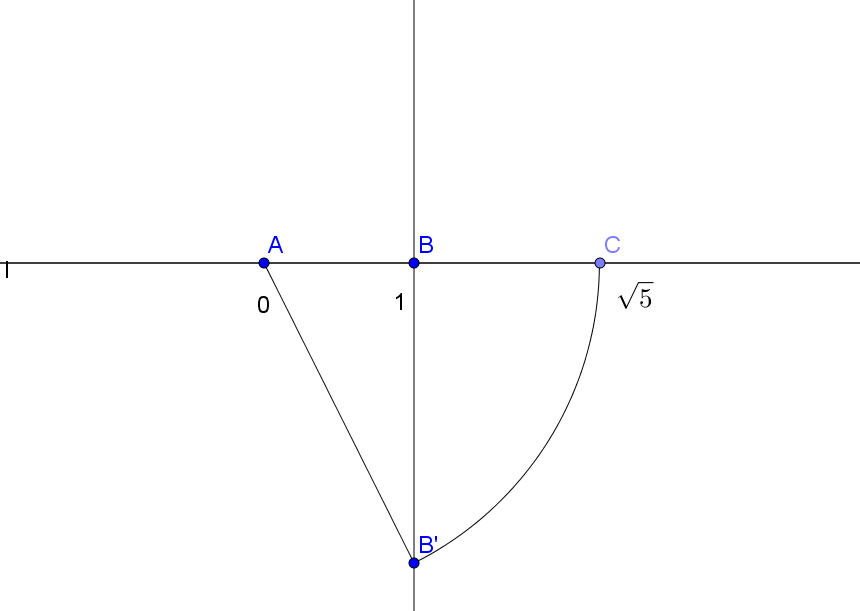
\includegraphics[width=.5\linewidth]{4_opp_inhoud_an_meetk/inputs/AMTekst1Fig8}
\caption{Constructie vierkantswortel van een natuurlijk getal (2).}
\label{4.2.1_fig_reeel_fig2}
\end{center}
\end{figure}

Algemeen kan voor ieder positief rationaal getal het punt op $l$ dat overeenkomt met de vierkanstwortel geconstrueerd worden.

Wiskundig kan aangetoond worden dat je het punt dat op $l$ overeenkomt met $\sqrt[3]{2}$ niet op soortgelijke wijze kunt construeren.
Ook een re\"eel getal zoals $\pi$ kun je niet op $l$ construeren.\vspace{2mm}

\noindent \underline{Definitie:} Voor een punt $P$ op $l$ noem je het re\"ele getal $x$ dat met $P$ overeenkomt de abscis van $P$ en je schrijft $\ab (P)=x$.

\begin{figure}[ht]
\begin{center}
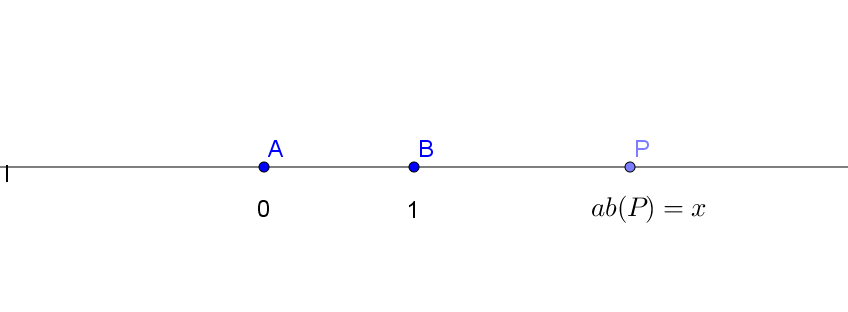
\includegraphics[height=3 cm]{4_opp_inhoud_an_meetk/inputs/AMTekst1Fig9}
\end{center}
\end{figure}

Merk op dat je pas over de abscis van een punt op een rechte kunt spreken nadat een ijk op de rechte vastgelegd is.\vspace{2mm}

\noindent \underline{Voorbeeld} 
%(Mijn voorstel is om dit voorbeeld uit leggen met lightboard.)
$l$ is een geijkte rechte met ijk $(A;B)$.
$B'$ is het punt op $l$ met $\ab (B')=-\frac{4}{3}$ en $P$ is het punt op $l$ met $\ab (P)=\frac{12}{5}$.
Wat is de abscis van $P$ als je op $l$ de ijk $(A;B')$ neemt?

\begin{figure}[ht]
\begin{center}
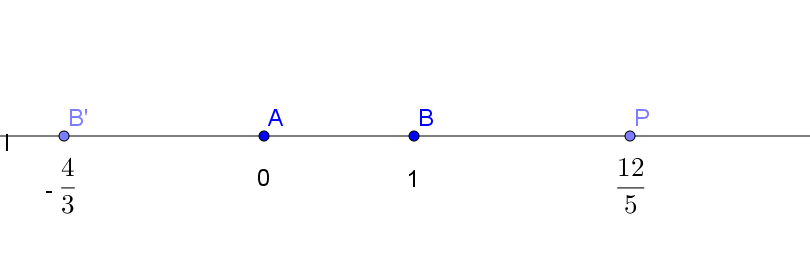
\includegraphics[height=3 cm]{4_opp_inhoud_an_meetk/inputs/AMTekst1Fig10}
\end{center}
\end{figure}

Het kleinste gemeenschappelijk veelvoud van 3 en 5 is 15.
Met deze noemer bekom je $\ab (B')=-\frac{20}{15}$ en $\ab (P)=\frac{36}{15}$.
De afstand van $P$ tot $A$ is $\frac{36}{15}.\frac{15}{20}=\frac{36}{20}$-ste van de afstand van $A$ tot $B'$.
Omdat $P$ aan de andere kant van $A$ ligt als $B'$ is de abscis van $P$ ten opzichte van de ijk $(A;B')$ gelijk aan $-\frac{36}{20}=-\frac{9}{5}$.

\begin{figure}[h]
\begin{center}
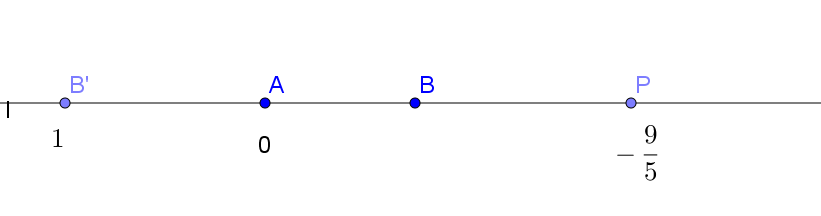
\includegraphics[height=3 cm]{4_opp_inhoud_an_meetk/inputs/AMTekst1Fig11}
\end{center}
\end{figure}

Kies een vaste lengte-eenheid (bijvoorbeeld 1 cm) .
Op een rechte $l$ kies je een ijk $(A;B)$ zodat de afstand van $A$ tot $B$ gelijk is aan die lengte-eenheid.
Je zegt dat de geijkte rechte dan overeenkomt met de lengte-eenheid.

Op een geijkte rechte $l$ die overeenkomt met de lengte-eenheid kies je twee punten $P$ en $Q$.
De afstand van $P$ tot $Q$ is dan het verschil tussen de abscissen $\ab (P)$ en $\ab (Q)$.
Noteer $d(P;Q)$ voor de afstand van $P$ tot $Q$.
Je bekomt in dat geval:
\[
d(P;Q)=\vert \ab (Q) - \ab (P) \vert \text { .}
\]

